\section{ANALISIS E INTERPRETACION DE RESULTADOS} 


\subsection{ Actividades Encargadas}
	\begin{itemize}
		\item ¿Con qué comando(s) puedo iniciar y detener una instancia de Oracle, detalle cada uno de los pasos y opciones,
utilizando Docker?
                     \item Para  Iniciar una instancia de Oracle Database Server
Iniciar una instancia de servidor de base de datos Oracle al ejecutar
" docker run -d -it --name oracle-db store/oracle/database-enterprise:12.2.0.1"donde oracle01-db está el nombre del contenedor y 12.2.0.1 es la etiqueta de imagen de Docker.
                      \begin{figure}[H]
		\begin{center}
		
\includegraphics[width=15cm]{./Imagenes/200}
		\end{center}
		\end{figure}
                      \item Los comandos docker ps -a -q detendrá todos los contenedores Docker en ejecución :
                      \begin{figure}[H]
		\begin{center}
		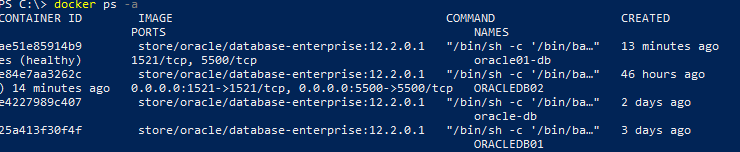
\includegraphics[width=15cm]{./Imagenes/201}
                      
\includegraphics[width=8cm]{./Imagenes/202}
		\end{center}
		\end{figure}
		\item ¿Con qué comando(s) puedo iniciar y detener el Listener y el Enterprise manager, detalle cada uno de los pasos y
opciones, utilizando Docker?
                     \item Parar iniciar el listener:" lsnrctl start"  para detener "lsnrctl stop"
                      \begin{figure}[H]
		\begin{center}
		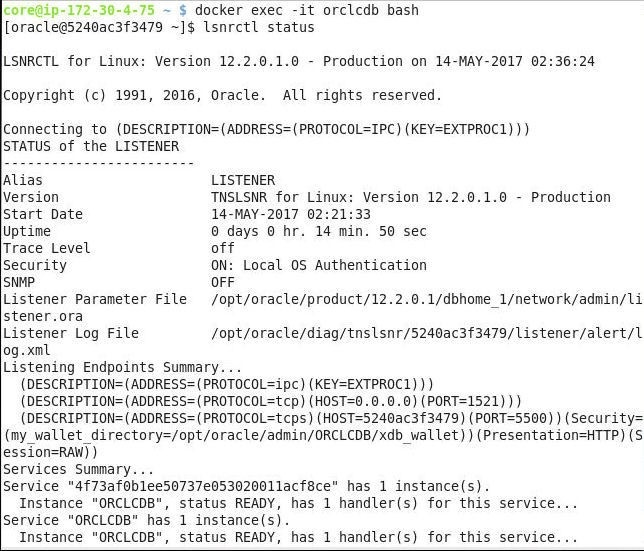
\includegraphics[width=15cm]{./Imagenes/203}
                      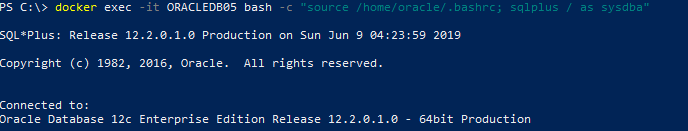
\includegraphics[width=15cm]{./Imagenes/204}
		\end{center}
		\end{figure}
		\item Genere un nuevo contenedor y cree un espacio de tablas con las siguientes características.
		\begin{figure}[H]
		\begin{center}
		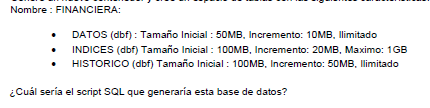
\includegraphics[width=8cm]{./Imagenes/t3}
		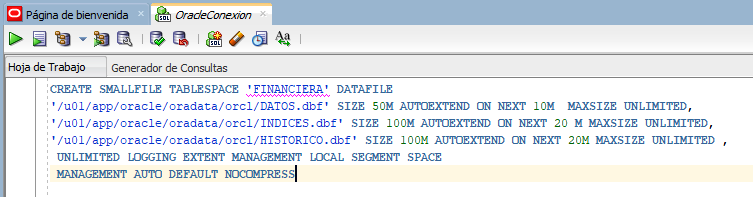
\includegraphics[width=15cm]{./Imagenes/23}
		\end{center}
		\end{figure}


	\end{itemize}



